\section{Global analysis and Conclusion}\label{Sec:glob_anal_conclusion}
In this section, as the authors did for the sake of convenience in representing the figures, I will change the order of the variables from $(K,E,L)$ into $(E,K,L)$.

In the following I take into consideration the case where, for $\alpha+\gamma<1$, two stationary states exist, $P_1^* = (E_1^*,K_1^*,L^*)$ and $P_2^* = (E_2^*,K_2^*,L^*)$, with $E_1^* < E_2^*$, $K_1^* < K_2^*$, $L^* = \frac{\beta}{\beta+\epsilon}$, and $P_1^*$ is a sink (when $\bar{E}$ is chosen properly in order to avoid Hopf bifurcation).

Hence the basin of attraction of $P_1^*$ can be considered a \textit{poverty trap} and I wonder if, given a point $P_0 = (E_0,K_0,L_0)$ belonging to such a basin, it is possible to modify the initial choice of labor $L_0$ in such a way that the positive semi-trajectory starting from the \textit{new} point $\widetilde{P}_0 = (E_0,K_0,\widetilde{L}_0)$ can tend to the saddle $P_2^*$ (having a two-dimensional stable manifold).

In fact, I will give a (partially) affirmative answer to the above question (Theorem \ref{thm:10_neighbor_of_P1_inters_manifold_P2}) and, moreover, I will conduct some numerical simulations that are aiming at detecting trajectories leading to the desirable equilibrium, i.e. to the saddle $P_2^*$ (formalization in Lemma \ref{lemma:7_subdivision_of_phase_space}).

These results will be obtained through a partial description of the shape of the saddle-point two-dimensional stable manifold. A full description of such a manifold is usually very difficult or impossible. However, in a three-dimensional system, two-dimensional stable (or unstable) manifolds are separatrices between different regimes of the trajectories. Therefore, if one is able to detect, in a significant region of the phase space (in our case a sub-region of the plane $L = L^*$ where $\dot{L}>0$), a separatrix between two sets of points whose trajectories show different behavior, that may lead to relevant information on the manifold of interest. As I will show, this is, in fact, our case.

Consider the following theorem.
\begin{thm} \label{thm:6_attracting_limit_pnt}
	Consider a point $P_0 = (E_0,K_0,L_0)$, $0<E_0<\bar{E}$, $0<K_0$, $0<L_0<1$. Then, if $L_0$ is small enough, the positive semi-trajectory from $P_0$ tends to $(\bar{E},0,0)$.
\end{thm}
\begin{proof}
	See in the paper \cite{antoci_poverty_2011}, pg. 582.
\end{proof}
As I said (and authors of the paper said), we want to see if, given a point $P_0 = (E_0,K_0,L_0)$ belonging to the basin of attraction of $P_1^*$ and sufficiently close to $P_1^*$, it is possible to modify the initial choice of labor in such a way that the positive semi-trajectory starting from the \textit{new} point $\widetilde{P}_0 = (E_0,K_0,\widetilde{L}_0)$ can tend to the saddle $P_2^*$. To this aim, as suggested by the above theorem I will consider values $\widetilde{L}<L_0$. For instance, let us start, in order to fix ideas, from $P_1^*$ itself. Moving downward along the half-line $E = E_1^*$, $K = K_1^*$, $L < L^*$, we cross, as shown in the above theorem, the basin of attraction of $P_1^*$ at a certain point, say $\widetilde{P}=(E_1^*,K_1^*,\widetilde{L})$, $\widetilde{L}<L^*$. I wonder if the positive
semi-trajectory starting from $\widetilde{P}$ tends to the saddle $P_2^*$. As $K_1^*<K_2^*$ and $K(t)$ decreases when $L<L^*$, the trajectory from $\widetilde{P}$, in order to tend to $P_2^*$, must cross, first, the plane $L = L^*$. In such a case, that will take place at a point where $K<K_1^*$ and $\dot{L}>0$.

Furthermore, observe that, being $\widetilde{L}<L^*$, $\dot{E}>0$ at $\widetilde{P}$. Should the trajectory \textit{go back}, before crossing $L = L^*$, to a point where $E= E_1^*$, at such a point it would be again $\dot{E}>0$, since $K<K_1^*$ and $L<L^*$. So our hypothetical trajectory must cross $L = L^*$ at a point where $E>E_1^*$
and $K<K_1^*$. 

The following lemma allows, precisely, to detect the points with the above described features, i.e. such that $E > E_1^*$, $K < K_1^*$, $L = L^*$, $\dot{L}>0$, belonging to the stable manifold of $P_2^*$.
\begin{lemma}\label{lemma:7_subdivision_of_phase_space}
	Let $\alpha+\gamma<1$ and assume that two equilibria exist, $P_1^* = (E_1^*, K_1^*, L^*)$ and $P_2^* = (E_2^*, K_2^*, L^*)$, $E_1^* < E_2^*$, $K_1^* < K_2^*$, $L^*=\frac{\beta}{\beta+\epsilon}$. Moreover, assume that the conditions of Lemma \ref{lemma:3_condition_for_simga_pos} of the previous section, i.e. $$\eta\geq \frac{\epsilon}{\epsilon+\alpha\beta},\quad  \bar{E}>E_B=\frac{\theta(\beta+\epsilon)(2-2\alpha-\gamma)}{\alpha\beta\gamma\eta}$$ are satisfied and that $P_1^*$ is a sink. Consider, in the plane $L=L^*$, the open set
	$$A = \{P = (E,K,L^*): E > E_1^*, K < K_1^*, \dot{L}(P)>0\}.$$
	Then A can be partitioned into three non-empty pair-wise disjoint subsets, $A=A_1 \cup A_2 \cup A_3$, where $A_1$ and $A_2$ are open, while $A_3$ is a unidimensional set belonging to the stable manifold of $P_2^*$. More precisely:
	
	$A_1$ is the subset of points $P\in A$ such that the positive semi-trajectory starting from $P$ crosses $\dot{E}=0$ before crossing again $L = L^*$.
	
	$A_2$ is the subset of points $Q\in A$ such that the positive semi-trajectory starting from $Q$ crosses again $L = L^*$ before crossing $\dot{E}=0$.
\end{lemma}
\begin{proof}
	See in the paper \cite{antoci_poverty_2011}, Appendix B.
\end{proof}
An immediate consequence of the previous lemma is the following:
\begin{corollary}
	Let $\alpha+\gamma<1$ and two equilibria, $P_1^*$ and $P_2^*$, exist, $P_1^*$ being a sink. Moreover, assume $\eta\geq \frac{\epsilon}{\epsilon+\alpha\beta}$ and $\bar{E}>E_B=\frac{\theta(\beta+\epsilon)(2-2\alpha-\gamma)}{\alpha\beta\gamma\eta}$. Then $P_2^*$ is a saddle with a two-dimensional stable manifold and the eigenvalues of its Jacobian matrix are all real (one positive and two negative).
\end{corollary}
\begin{remark}
	\textup{The above corollary suggests that, in the case of two fixed points, whenever $P_1^*$ is a sink, the eigenvalues at $P_2^*$ are all real: one positive and two negative. However, it happens that, when $P_1^*$ is not attracting, $P_2^*$ can be either a saddle-point with two negative real part complex eigenvalues or a source (all eigenvalues have positive real part).}
\end{remark}
For example, I shall adopt the above notations and I recall from the proof of the Theorem \ref{thm:result_of_analysis} that $E_C := \frac{b(2-2\alpha-\gamma)}{1-\alpha-\gamma}$ where $b$ is defined in \eqref{eqn:a_b_def}, and $E_A$ from \eqref{eqn:E_A}. I assume, firstly, 
$E_A=E_C>\widehat{E}:=\frac{\theta(1-\alpha)(\beta+\epsilon)(2-2\alpha-\gamma)}{\alpha\gamma[\eta(\beta+\epsilon)-\epsilon]},\ a=0$.\\
Then it is easily checked that, if $0<\bar{E}-E_A\ll 1$, \\
$trace(J(P_2^*))<0<trace(J(P_1^*))$, $det(J(P_1^*))<0<det(J(P_2^*))$ and\\
$|trace(J(P_{1,2}^*))|\ll \sigma(J(P_{1,2}^*))$ hold.\\
This implies that $P_1^*$ has one negative and two positive real part complex eigenvalues, while $P_2^*$ has one positive and two negative real part complex eigenvalues.

Vice versa, let, with the same notations, $E_C>E_A>\widehat{E},\ a=0.$ Then, if $0<\bar{E}-E_A\ll 1$, both $trace(J(P_1^*))$ and $trace(J(P_2^*))$ are positive,\\ $det(J(P_1^*))<0<det(J(P_2^*))$ and $\rho(J(P_2^*))<0$.\\
Hence in this case $P_1^*$ has again a one-dimensional stable manifold, while $P_2^*$ is a source (three positive real part eigenvalues). Moreover, when, posed $E_A=\lambda\widehat{E}+(1-\lambda)E_C$, $0<\lambda<1$, and $\lambda$ sufficiently small, then both $P_1^*$ and $P_2^*$ have two complex conjugate eigenvalues.

At this point, one is able to prove the main theorem: 
\begin{thm}\label{thm:10_neighbor_of_P1_inters_manifold_P2}
	Given the assumptions of Lemma \ref{lemma:7_subdivision_of_phase_space}, there exists a neighborhood N of the sink $P_1^*$, such that, for any $(E_0,K_0,L_0)\in N$, the half-line \\$\{E=E_0,K = K_0,L < L_0\}$ intersects the stable manifold of $P_2^*$.
\end{thm}
\begin{proof}
	See in the paper \cite{antoci_poverty_2011}, pg. 584. 
\end{proof}
\begin{figure}[h!]
	\centering
	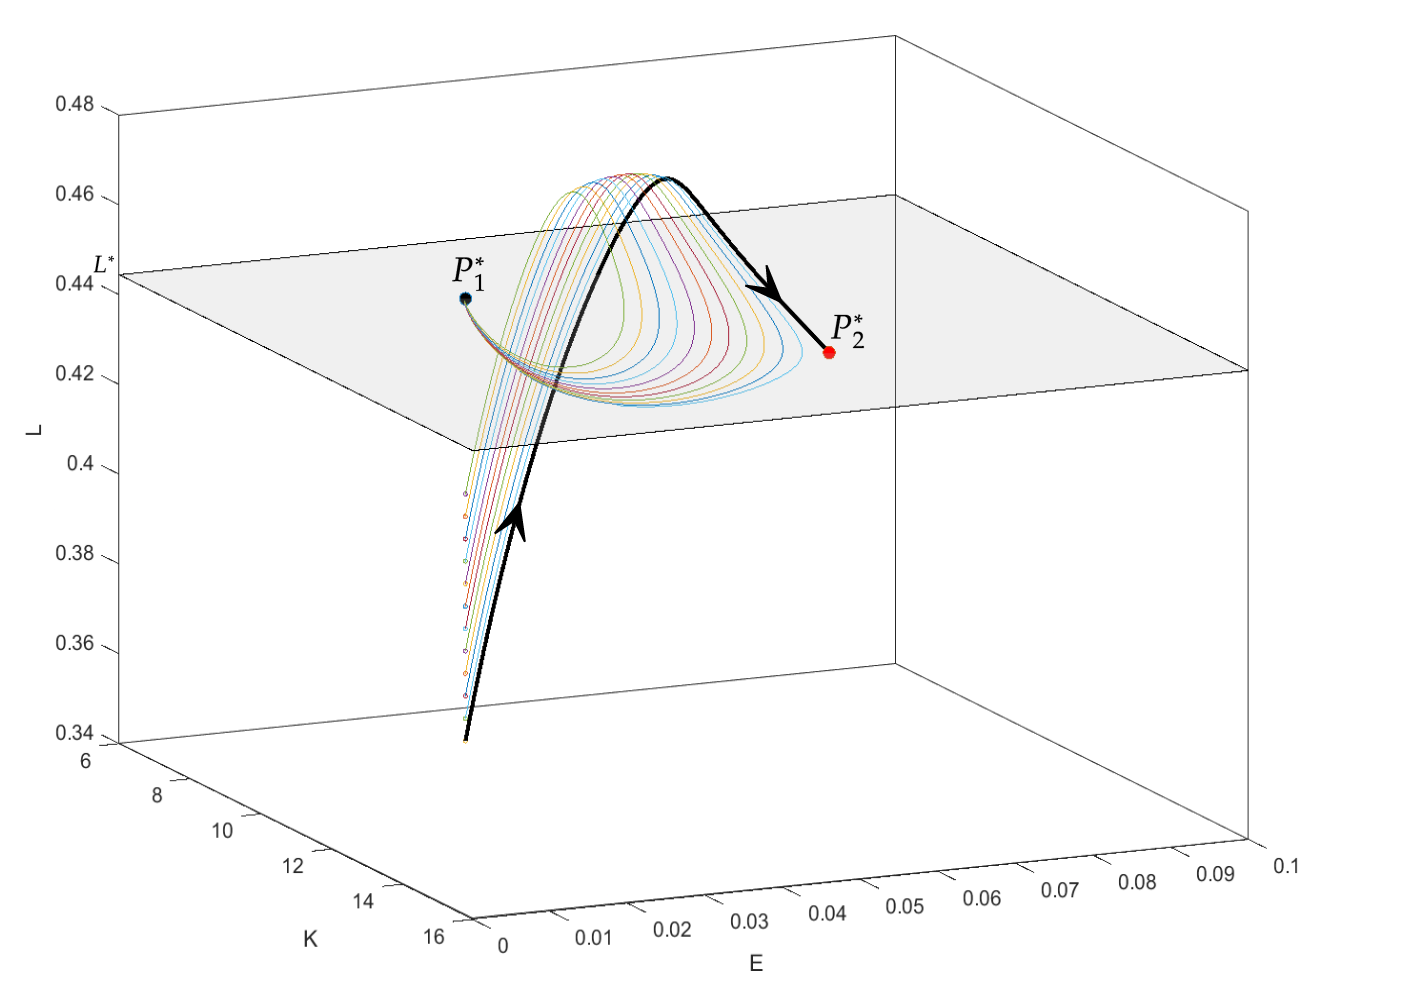
\includegraphics[width=1.\linewidth]{global_indeterminacy.png}
	\caption{Global indeterminacy in the space ($E,K,L$); the black trajectory (in bold) approaching $P_2^*=(E_2^*,K_2^*,L^*=0.444444)$ starts from the point $(E_1^*,K_1^*,L_0\simeq 0.345910588598)$; parameter values: $\alpha=0.1$, $\beta=0.8$, $\gamma=0.58$, $\delta=0.05$, $\epsilon=1$, $\eta=1.5$, $\theta=0.001$, $\bar{E}=0.17$.}
	\label{fig:global_indeter}
\end{figure}
\begin{figure}[h!]
	\centering
	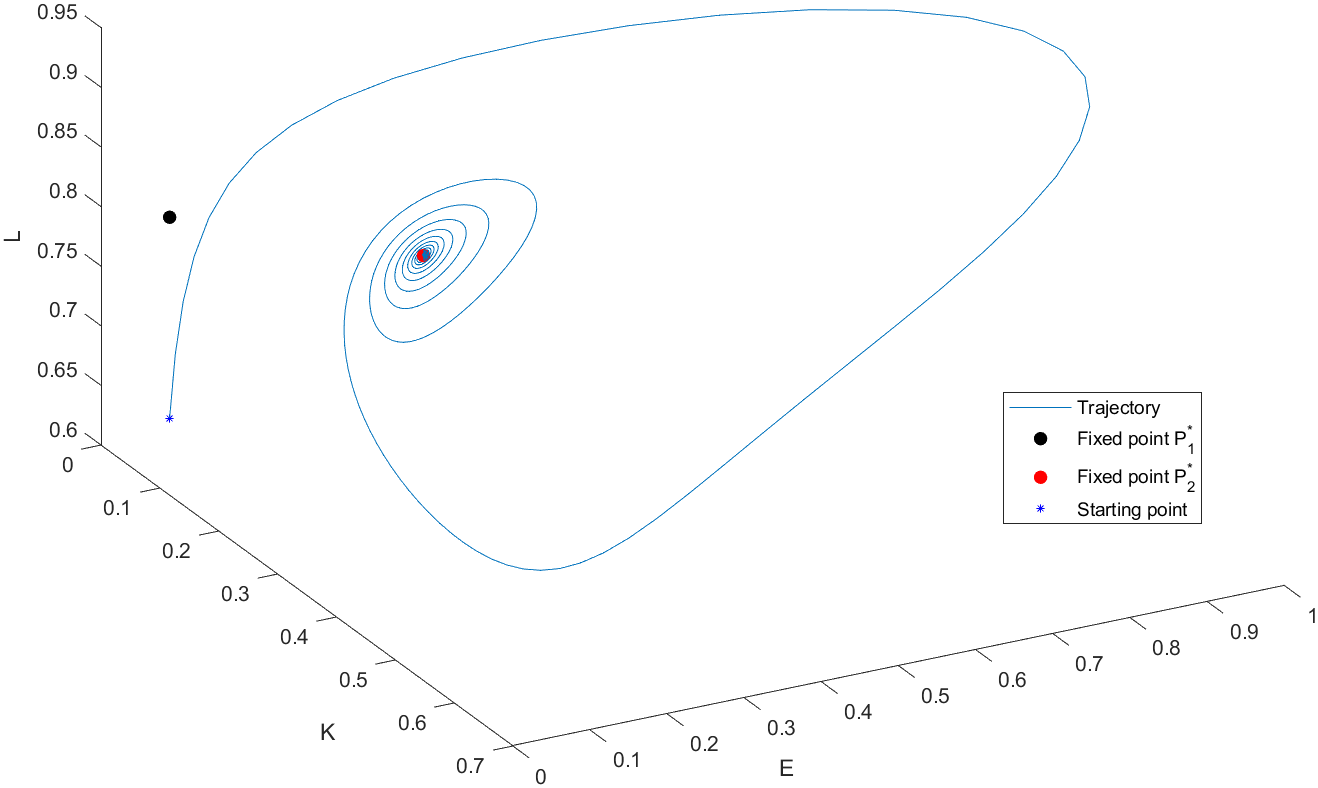
\includegraphics[width=.8\linewidth]{traj_spiraling_to_P2.png}
	\caption{A trajectory spiraling toward $P_2^*$ starting from the point ($E_1^*,K_1^*,L_0 \simeq 0.6316546$) plotted with a low end time $(T=100)$; parameter values: $\alpha=\theta=0.19$, $\beta=\gamma=0.8$, $\epsilon=0.2$, $\eta=\frac{4}{9}$, $\delta=12.8620934285269$, $\overline{E}=10.75$.}
	\label{fig:traj_spiral_P2}
\end{figure}
\begin{figure}[h!]
	\centering
	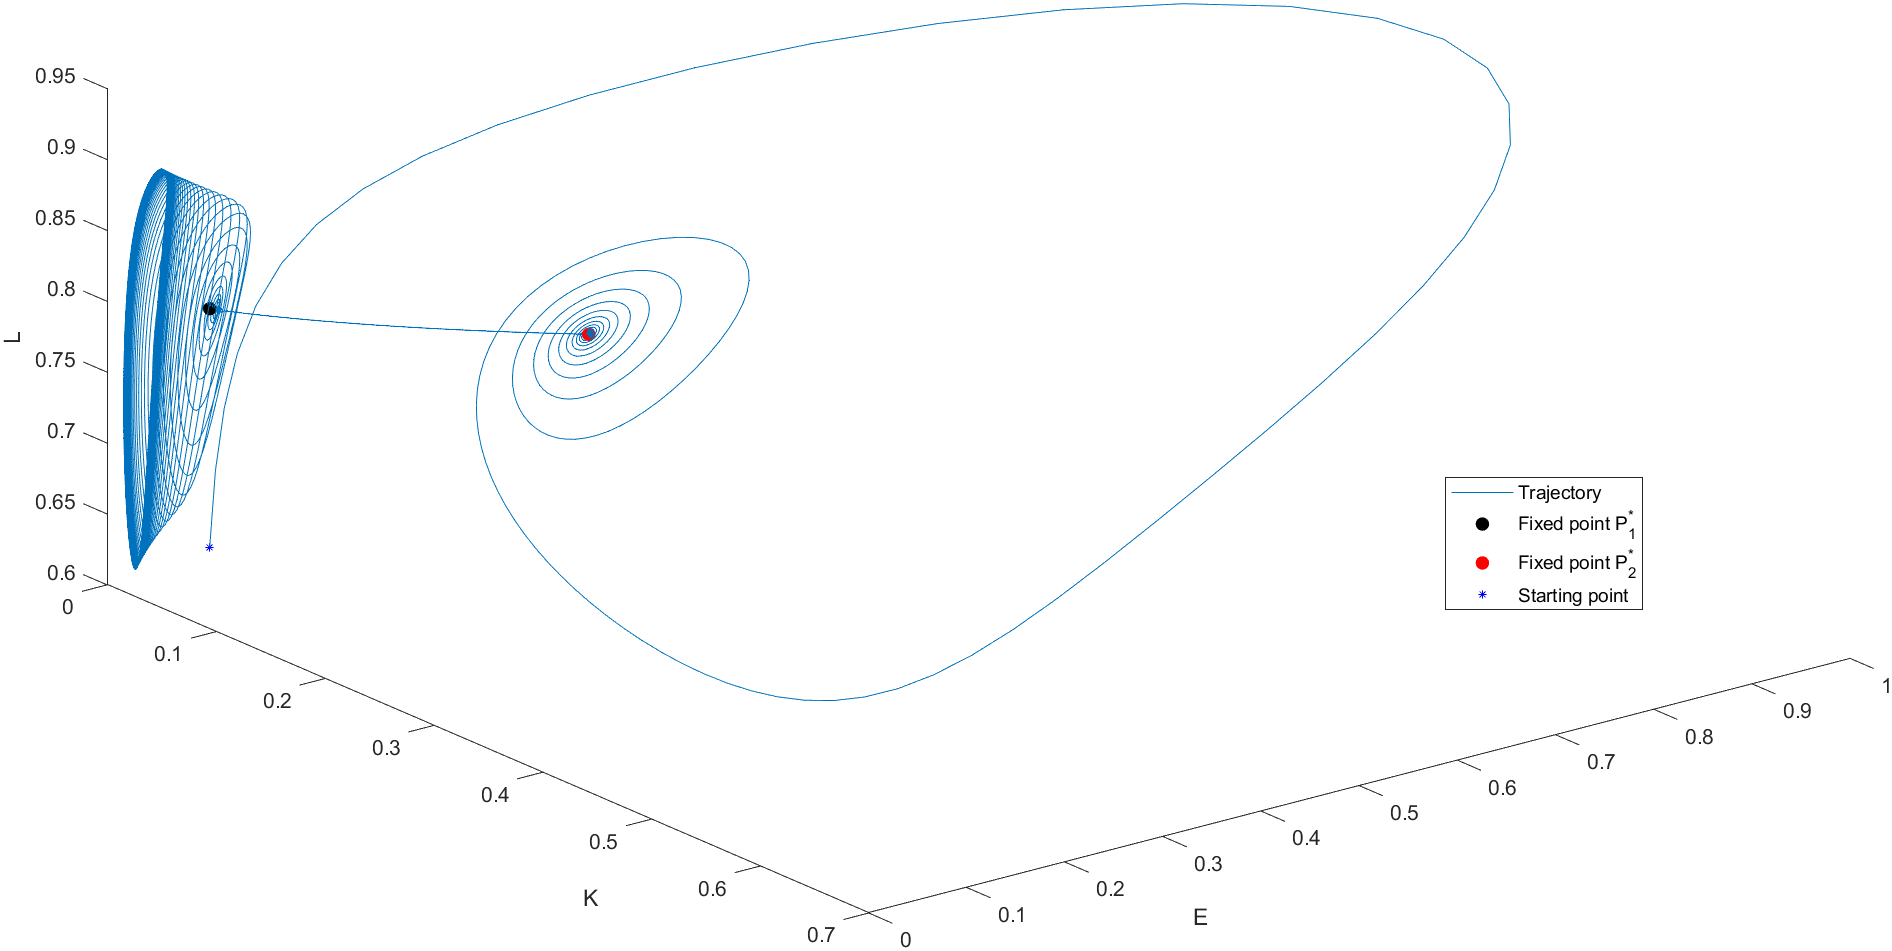
\includegraphics[width=.8\linewidth]{traj_spiraling_to_P2_with_limit_cycle_P1.png}
	\caption{The same trajectory spiraling toward $P_2^*$ starting from the point ($E_1^*,K_1^*,L_0 \simeq 0.6316546$) as in Figure \ref{fig:traj_spiral_P2} but plotted with a high end time $(T=1000)$; the same parameter values.}
	\label{fig:traj_spiral_P2_with_limit_cycle_P1}
\end{figure}
\begin{figure}[h!]
	\centering
	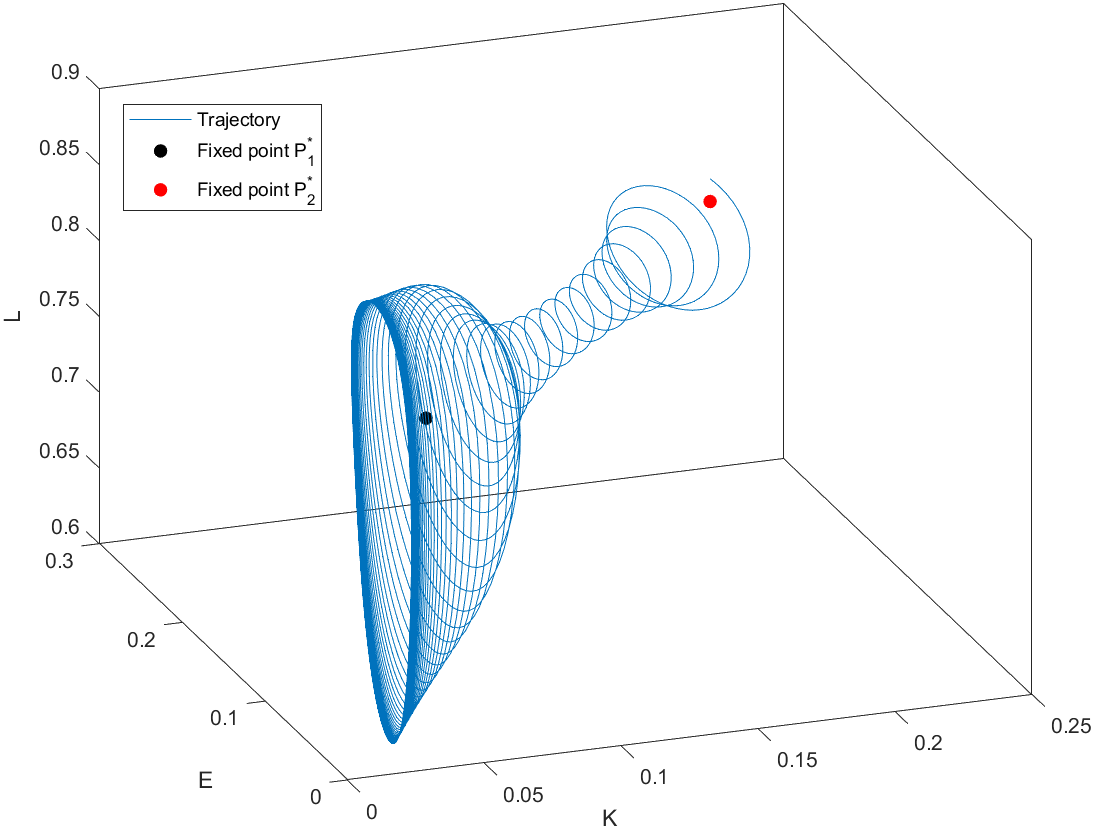
\includegraphics[width=.8\linewidth]{from_P2_to_limit_cycle_P1.png}
	\caption{Starting from the point $(E_2^*,K_2^*,L_0 \simeq 0.815)$, "very close" to $P_2^*=(E_2^*,K_2^*,L^*=0.8)$, the trajectory approaches the attracting limit cycle surrounding $P_1^*$; the parameter values are those used in Figure \ref{fig:traj_spiral_P2}.}
	\label{fig:from_P2_to_limit_cycle_P1}
\end{figure}
Therefore, under the assumptions of the theorem, for any initial point $(E_0, K_0)$ sufficiently close to $(E_1^*, K_1^*)$, there exists a continuum of initial values $L_0^1$ such that the trajectory starting from $(E_0, K_0, L_0^1)$ approaches $P_1^*$, and a locally unique value $L_0^2$ such that the trajectory starting from $(E_0, K_0,L_0^2)$ converges to $P_2^*$. So global indeterminacy occurs, since, from the initial position $(E_0, K_0)$, the economy may follow one of the trajectories belonging to the basin of attraction of the 'poverty trap' $P_1^*$ but it may also follow a trajectory lying on the stable manifold of the stationary state $P_2^*$.

In Figure \ref{fig:global_indeter} a numerical simulation is shown. The starting points of the trajectories are chosen along the half-line $\{E=E_1^*, K=K_1^*, L<L^*\}$. The trajectory in bold lies on the stable manifold of $P_2^*$ and consequently converges to $P_2^*$, while all the others approach $P_1^*$. Notice that some trajectories approaching $P_1^*$ are characterized by an initial phase where the values of $K$ and $L$ are higher than along the trajectory converging to $P_2^*$; however, the higher values of $K$ and $L$ give rise to over-exploitation of the natural resource and the consequent reduction of the stock $E$ drives the economy towards the undesirable equilibrium $P_1^*$, where the values of $K$ and $E$ are lower than in $P_2^*$.
\begin{figure}[h!]
	\centering
	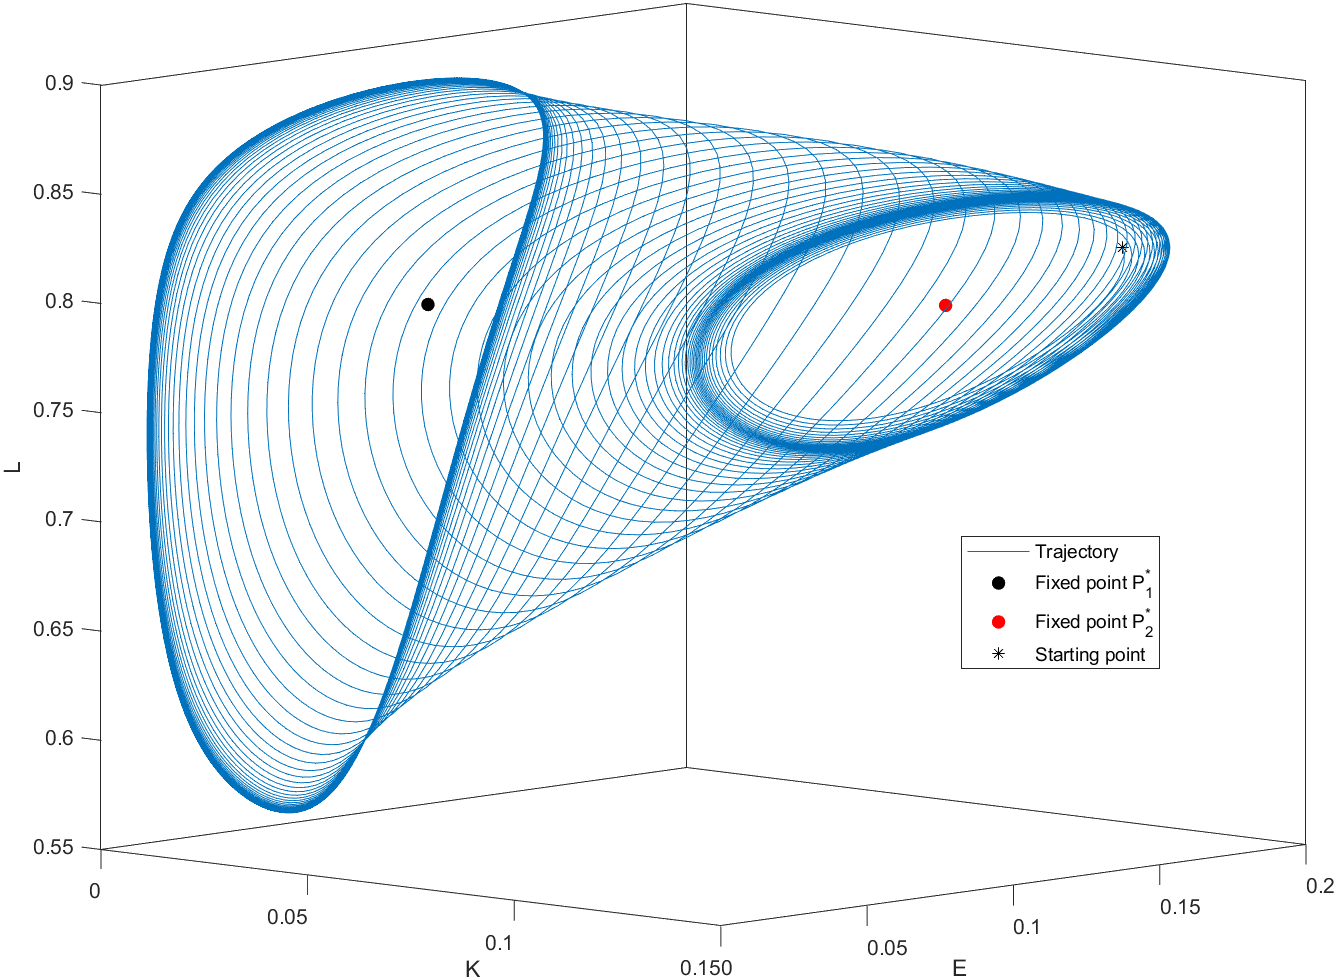
\includegraphics[width=.8\linewidth]{two_limit_cycles_P1_and_P2.png}
	\caption{Two limit cycles: an attractive one “around” $P_1^*$ and a repulsive one “around” $P_2^*$; parameter values: $\alpha=\theta=0.19$, $\beta=\gamma=0.8$, $\epsilon=0.2$, $\eta=\frac{4}{9}$, $\delta=8.42228$, $\overline{E}=7.06$.}
	\label{fig:2_limit_cycles_P1_and_P2}
\end{figure}

In the main model studied in this work, global indeterminacy can occur even if the assumptions of Lemma \ref{lemma:7_subdivision_of_phase_space} are not satisfied, as the trajectories drawn in Figures \ref{fig:traj_spiral_P2}-\ref{fig:from_P2_to_limit_cycle_P1} suggest.

In those figures, $P_1^*=(E_1^*,K_1^*,L^*)$ has one negative and two positive real part complex eigenvalues, while $P_2^*$ has one positive and two negative real part complex eigenvalues (computed with the already implemented code setting properly the parameters, see appendix \ref{app:A}). Numerical simulations suggest the existence of an attracting limit cycle surrounding $P_1^*$. \\
In Figure \ref{fig:traj_spiral_P2} the
point $(E_1^*,K_1^*,L_0)$, lying on the half-line $\{E = E_1^*,\ K = K_1^*,\ L < L^*\}$, appears to belong to the stable manifold of $P_2^*$ (i.e. the trajectory starting from it approaches $P_2^*$). In case one performs the simulation for particularly long time (e.g. $T=1000$), it can be observed that the spiraling around $P_2^*$ goes to a limit cycle around $P_1^*$ as shown in the Figure \ref{fig:traj_spiral_P2_with_limit_cycle_P1}.\\
Using the same parameter values of Figure \ref{fig:traj_spiral_P2}, the simulation in Figure \ref{fig:from_P2_to_limit_cycle_P1} shows a trajectory starting from a point on the half-line $\{E = E_2^*, K = K_2^*, L > L^*\}$, very close to the saddle-point $P_2^*$, which approaches the attracting limit cycle surrounding $P_1^*$.

Figure \ref{fig:2_limit_cycles_P1_and_P2} shows the occurrence of two limit cycles. In this case $P_1^*$ has one negative and two positive real part complex eigenvalues, while $P_2^*$ is a source (three positive real part eigenvalues). The simulation shows an attracting limit cycle surrounding $P_1^*$ and a not-attracting one arisen around $P_2^*$ through a Hopf bifurcation and endowed with a two-dimensional stable manifold, which bounds, as a separatrix, the basin of the attracting limit cycle.